\documentclass[a4paper]{article}

% Import packages.tex
% PACKAGES

% Input UTF-8 characters
\usepackage[utf8]{inputenc}
% Typographical rules and hyphenation patterns
\usepackage[english]{babel}
% Clickable links, also in TOC
\usepackage{hyperref}
% Environments framed, shaded and leftbar
\usepackage{framed}
% Set all page margins to 1.5cm, option 'headings' sets \pagestyle{headings}
\usepackage[headings]{fullpage}
% Set of math symbols
\usepackage{amssymb}
% Use Latin Modern font
\usepackage{lmodern}
% Floating algorithm environment with algorithmic keywords
\usepackage[linesnumbered,onelanguage,ruled,lined]{algorithm2e}
% H (here) float mod­i­fier op­tion
\usepackage{float}
% Extra Arrows beyond those provided in amsmath
\usepackage{extarrows}
% Caption alignment
\usepackage{caption}

% TIKZ

% For creating graphics programmatically
\usepackage{tikz}
% Automata and relative positioning
\usetikzlibrary{automata,positioning}

% Theorem setup

\usepackage{amsthm}
% Definition environment with numbered with subsection.
\theoremstyle{definition}
\newtheorem{definition}{Definition}[subsection]


\begin{document}
	\title{\LaTeX\ Science Template}
	\author{Author 1 \and Author 2}
	\maketitle
	
	\pagebreak
	
	\tableofcontents
	\pagebreak
	
	\section{Useful snippets}
	
	\subsection{Math}
	Let's write some random math.
	% Some math on a new line
	\[ \bigcup_{i=0}^{n} x_i \indent n \in \mathbb{N} \]
	And an aligned equation.
	% Aligned equation
	\begin{equation}
		\begin{split}
			P &= NP\\
			&\vee \\
			P&\neq NP
		\end{split}
	\end{equation}
	
	\subsection{Algorithm}
	\begin{algorithm}[H]
		$R:=\emptyset$\;
		$L(a):=0$\;
		$\forall v\neq a:L(v):=\infty$\;
		\While{$z\notin R$}{
			choose $v\in V\backslash R$ with lowest $L(v)$\;
			$R:=R\cup\{v\}$\;
			\ForEach{edge $(v,v')\in E$ with $v'\in V\backslash R$}{
				$L(v'):=min\{L(v)+w(v,v'),L(v')\}$
			}
		}
		\caption{Dijkstra's shortest path algorithm}
	\end{algorithm}
	
	\subsection{Definition \& proof}
	\begin{leftbar}
		\begin{definition}[Example definition]
			A definition, nicely wrapped by a \texttt{leftbar} environment.
		\end{definition}
	\end{leftbar}
	\begin{proof}
		Of course, we can't leave the proof out.
	\end{proof}
	
	\subsection{Figure}
	Let's see what \autoref{fig:plots} looks like. ``Figure 1" in the previous sentence is a clickable reference.
	% Using the H modifier from the float package to include the figure HERE.
	\begin{figure}[H]
		% Center figure
		\centering
		% Center caption
		\captionsetup{justification=centering}
		% The actual figure
		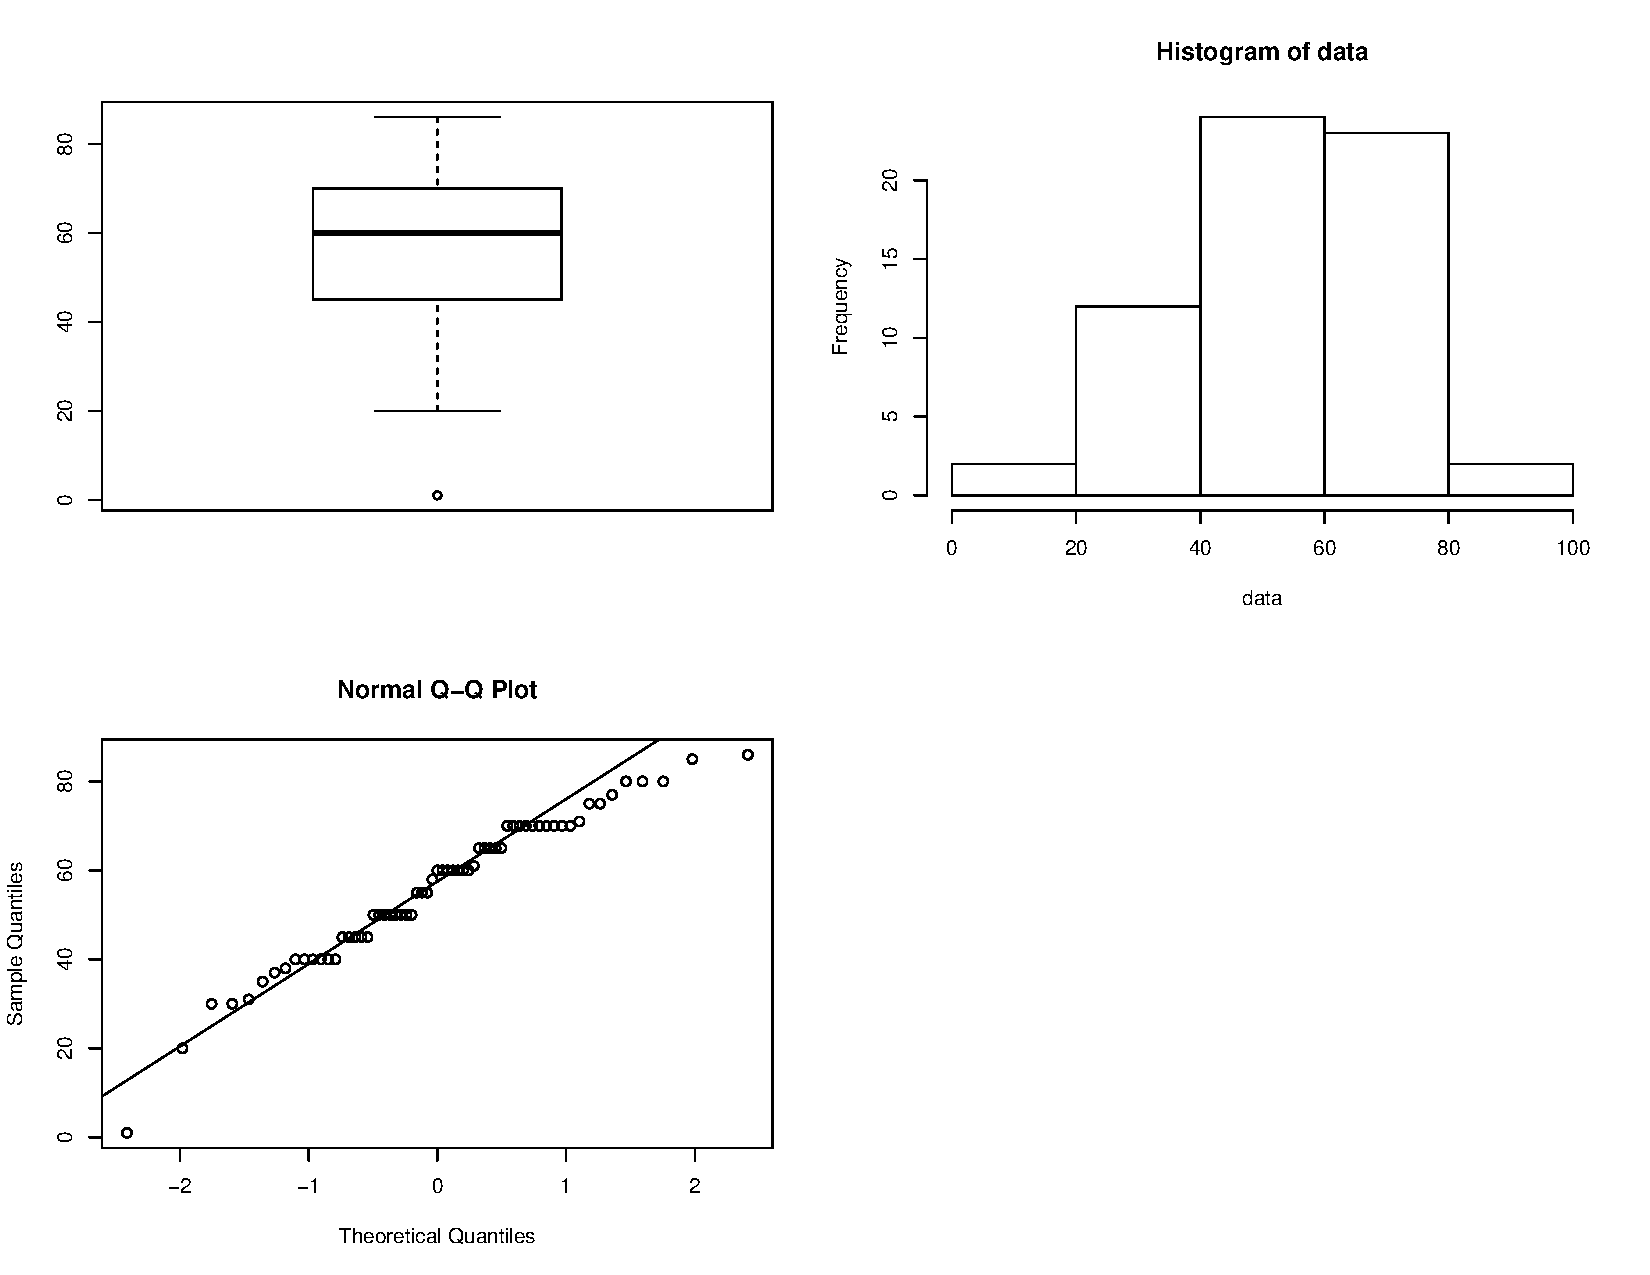
\includegraphics[scale=0.2]{assets/plots}
		% And a nice caption
		\caption{Example of including an image in a \LaTeX\ document, centered and positioned exactly where it's included in the code.\label{fig:plots}}
	\end{figure}
\end{document}
